\chapter{Word Embedding} \label{wordemb}
Documents are made by words.
To be manipulable by an algorithm these words need to be represented in a numerical format.

This chapter covers some techniques able to fulfil this task,
pointing out the advantages and disadvantages of choosing one instead of another.

To avoid misunderstandings
we define the term \say{word} as a word in a particular position in a document,
while we use the word \say{term} as a generic word into a dictionary.

For instance, given a document \say{A cat is an animal but an animal is not a cat} its list of words
is $ w = (a, cat, is, an, animal, but, an, animal, is, not, a, cat)$
while its set of terms is $d = \{a, cat, is, an, animal, but, not\}$.

\section{One Hot Encoding}
Given a list of words $w = (w_1, w_2, \dots, w_N)$,
we first generate a dictionary of unique terms
$d = \{d_1, d_2, ..., d_K\}$ with an arbitrary order between words.
Note that $ K \leq N $ is always true and $ K = N $ happens only when there is no repetition of words in the documents.

Each term $d_i$ in the dictionary can now be encoded as $x_i \in \{0,1\}^K$ following the One Hot Encoding approach.
All elements of $x_i$ are zero except a \say{1} in the position  $i$ of the vector.
That means that two words $w_l, w_j$ in different positions will have the same value $x_i$ if and only if they correspond to the same term $d_i$.

Applying One Hot Encoding on the previous example presented in the introduction of this chapter leads to the following values of $x_i$:
\begin{multicols}{2}
    \begin{itemize}
        \item $x_1 = x_{a} = [1, 0, 0, 0, 0, 0, 0]$
        \item $x_2 = x_{cat} = [0, 1, 0, 0, 0, 0, 0]$
        \item $x_3 = x_{is} = [0, 0, 1, 0, 0, 0, 0]$
        \item $x_4 = x_{an} = [0, 0, 0, 1, 0, 0, 0]$
        \item $x_5 = x_{animal} = [0, 0, 0, 0, 1, 0, 0]$
        \item $x_6 = x_{but} = [0, 0, 0, 0, 0, 1, 0]$
        \item $x_7 = x_{not} = [0, 0, 0, 0, 0, 0, 1]$
    \end{itemize}
\end{multicols}

Despite its simplicity and the fact that it is not computationally expensive to use, it has some disadvantages:
\begin{itemize}
    \item vectors are sparse: only one element of each vector is not zero
    \item there is no concept of similarity: all vectors have the same distance between each other
\end{itemize}

\section{Word2vec}
Word2vec is a family of approaches to overcome the disadvantages of One Hot Encoding using neural networks.
Originally presented in \cite{DBLP:journals/corr/abs-1301-3781}, it was later resumed by other authors due to the lack of details in the original paper.
For our document, we use \cite{DBLP:journals/corr/Rong14} as a reference.


In this section, two architectures are proposed.
Both of them should be trained using mini-batch gradient descent instead of gradient descent to allow the algorithm to scale when datasets grow in size.

After a learning phase, they will be able to map each term $x_i \in \{0, 1\}^K$ to a point $y_i \in \mathbb{R}^V$, with $V \ll K$.
Points in the new space will have a notion of similarity:
if two terms $d_l$ and $d_j$ appear in similar contexts and/or they have the same semantic content,
their vectors $y_l$ and $y_j$ will be close together.
On the opposite situation, $y_l$ and $y_j$ will be distant from each other.

For instance, $y_{cat}$ will probably be closer to $y_{dog}$ than $y_{computer}$.

\begin{figure}[ht]
    \centering
    \subfigure{\includegraphics[width=0.5\textwidth]{images/cbow.eps}}%
    \hfill
    \subfigure{\includegraphics[width=0.5\textwidth]{images/skip-gram.eps}}
    \caption{CBOW (left) and Skip-Gram (right) models with $K=3$ and $V=2$.}
    \label{fig:nnwemb}
\end{figure}

\subsection{Continuous Bag-of-Words Model (CBOW)}
First, the entire corpus is divided into contiguous blocks of words with odd length $N$ called n-grams.

Suppose to have the phrase \say{A cat is the best animal.} and n-grams of size $3$.
The corresponding blocks are:
\begin{multicols}{2}
    \begin{itemize}
        \item $(a, cat, is)$
        \item $(cat, is, the)$
        \item $(is, the, best)$
        \item $(the, best, animal)$
    \end{itemize}
\end{multicols}

The goal is to predict a word given its context.
For each n-gram, the CBOW neural network has as inputs all words in the block
except the one in the center which is used as ground truth for the classification task.
All words are encoded using the One Hot Encoding method.

For each n-gram, the first layer takes each input word encoded as $x_i \in \{0, 1\}^K$ and projects it into a smaller space $\mathbb{R}^V$
where $V$ is a hyperparameter to tune.
This is done through a shared matrix $M_{K \times V}$ which represents a fully connected layer.
Each projection is then averaged out with the others in the same block.
Note that in this way the order of the input words of the same sequence does not matter anymore.

The previous layer is then linked to a final layer in a fully connected way.
Since the classification task is on a One Hot Encoding vector,
a softmax activation function is used at the end.

Instead of using the network for the task for which it was trained, we use the matrix $M_{K \times V}$ to encode all terms as vectors in $\mathbb{R}^V$.

Note that there is no need to compute $M x_i$ for each $i$.
Since every $x_i$ has zero values everywhere except a \say{1} in the position $i$ of the vector, the result of the multiplication $M x_i$ is the $i$-th row $i$ the matrix M.
For this reason, each row $i$ of $M$ represents the term in position $i$ of the dictionary, encoded using CBOW.

An illustration of CBOW can be seen in Figure \ref{fig:nnwemb}.

\subsection{Continuous Skip-gram Model (Skip-gram)}
The Skip-gram model is the opposite approach of CBOW.

For each n-gram, the word in the center is fed to the neural network as the only input.

The second layer projects it to a smaller space through a matrix $M_{K \times V}$.
Unlike the previous model, there is no averaging since there is just one word as input.

Finally, the last layer tries to predict all remaining words of a block.
Each predicted word is obtained multiplying the hidden layer with a shared matrix $M'_{V \times K}$.
For each group of $K$ nodes which refers to a predicted word, we apply separately a softmax function.
To increase the accuracy, we can pick the number of output words less than $N-1$ and then sampling
words in the same phrase weighted by how distant they are from the input word.

If there are $N-1$ words to predict and each word is represented as a vector in $\mathbb{R}^K$,
the total number of nodes of the final layer is $(N-1)K$.

As previously, we use the matrix $M$ to encode each term $x_i$.

An illustration of Skip-Gram can be seen in Figure \ref{fig:nnwemb}.

\subsection{Interpretation of the results}
CBOW and Skip-Gram models are similar to Autoencoders,
with the difference that we are using the intermediate representations to predict words in the same phrase.
This leads to words having close values of $y$ if they appear often in the same context.

Furthermore, the paper \cite{DBLP:journals/corr/abs-1301-3781}
found out that these models go beyond syntactic regularities: for example,
the result of $y_{king} - y_{man} + y_{woman}$ is the closest vector to $y_{queen}$.
Note that subsequent papers like \cite{DBLP:journals/corr/abs-1905-09866} scale down the previous claim,
adding the constraint that no input vector can be returned by the prediction.

\section{Global Vectors (GloVe)}

GloVe was proposed in \cite{pennington2014glove} to overcome the limitations of Word2vec.
In particular, it builds a term-term co-occurrence matrix
to utilize the statistics of the entire corpus
instead of training the model on single n-grams.

Let  $X$ the term-term co-occurrence matrix.
$X_{ij}$ measures how many times the term $d_i$ occurs in the corpus near
the term $d_j$. Based on how you define the term \say{near},
the elements of the matrix will have different values.
For simplicity, we increment the counter ($X_{ij} = X_{ij} + 1$) every time
two terms appear in a phrase with less than $N$ words between them, with $N$ a
hyperparameter to tune. Given that, $X$ is symmetric.

An initial proposal could be to solve $ \min_{u,v} \sum_{i,j} (u_i^T v_j - X_{ij})^2$
in order to have vectors $u_i, v_j \in \mathbb{R}^V$ that have a high dot product if the terms $d_i$ and $d_j$
appear frequently together and vice versa.

We then apply the logarithm to $X_{ij}$:
\[ \displaystyle \min_{u,v} \sum_{i,j} (u_i^T v_j - log_2(X_{ij}))^2 \]
In this way, we lower the gap between frequent terms and rare ones.

The huge problem with this model is that all terms are weighted in the same way,
no matter how frequent they appear in the corpus.
To avoid this drawback, we introduce a weighting function $f(X_{ij})$ with the following characteristics:
\begin{itemize}
    \item $\boldsymbol{f(0) = 0}$: when $X_{ij} = 0$ the previous equation is undefined, while here the co-occurrence is not considered
    \item \textbf{$\boldsymbol{f}$ should be non-decreasing}: frequent terms must be considered more than rare ones
    \item \textbf{$\boldsymbol{f}$ needs to have a cutoff} to avoid weighting too much terms that appear often in the text and which do not convey semantic information.
          These terms are commonly called \say{stop words} in the literature. Examples are \say{the}, \say{a}, \say{from} and so on.
\end{itemize}
An illustration of a valid $f(X_{ij})$ can be viewed in Picture \ref{fig:glovef}.

After this addition, the minimization problem becomes:
\[ \displaystyle \min_{u,v} \sum_{i,j} f(X_{ij}) [u_i^T v_j - \log_2(X_{ij})]^2 \]

Consider that even the summation is over all combinations of terms,
the matrix is sparse and so the minimization is not as computationally intensive
as computing it on a dense matrix.

After taking gradient descent to resolve that minimization, we will obtain vectors
$u_j, v_j$ similar between each other because of the symmetricity of $X$.
Since $u_j \simeq v_j$, a reasonable choice for our new vector representation of
each term $d_j$ could be taking their average:
\[y_j = \frac{u_j + v_j}{2}\]

\begin{figure}[ht]
    \centering
    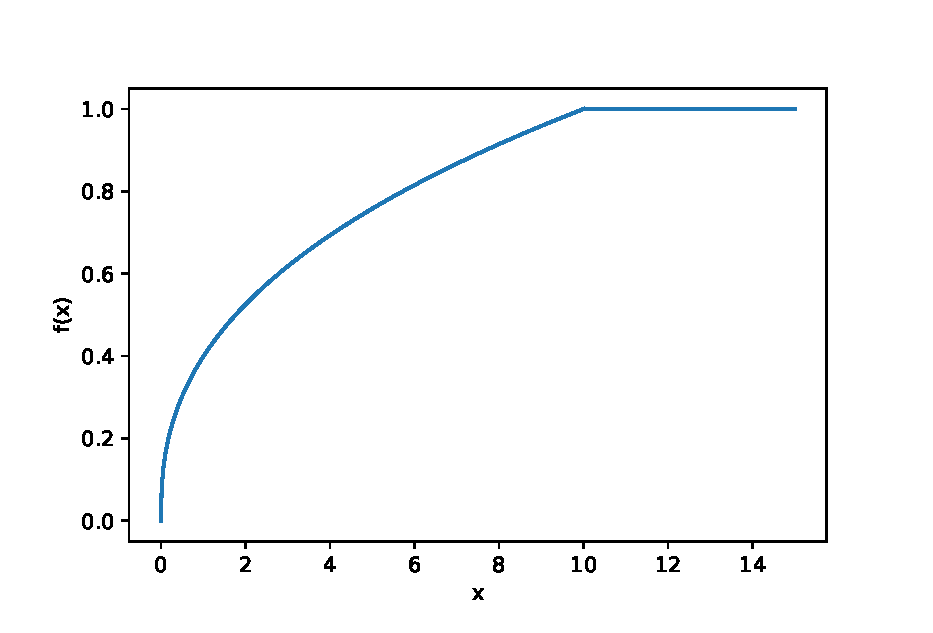
\includegraphics[width=0.5\textwidth]{images/glovef}
    \caption{Example of a valid $f(X_{ij})$ function for the minimization step of GloVe.}
    \label{fig:glovef}
\end{figure}

\section{Measuring distances between terms}
In the previous sections the term \say{close} was intentionally left vague.
Different distances between vectors could be considered.
In particular, we propose two of them:
\begin{itemize}
    \item \textbf{euclidian distance}: $\mathit{distance}(p, q) = \sqrt{\sum_i (p_i - q_i)^2}$
    \item \textbf{cosine similarity}: $\mathit{distance}(p, q) = \frac{p^T q}{\left\lVert p \right\rVert \left\lVert q \right\rVert} = \frac{\sum_i p_i q_i}{\sqrt{\sum_i p_i^2} \sqrt{\sum_i q_i^2}}$
\end{itemize}

While the first one measures the straight-line distance of two points, the second one returns the cosine of the angle between the corresponding vectors.

In the literature presented, the cosine similarity is the default choice to measure the closeness between terms.
One reason to prefer it instead of the euclidian distance
can be found in \cite{DBLP:journals/corr/SchakelW15}: the magnitude of the vector representation of a term
is correlated with the frequency of its appearance in the corpus which means that
a term with the same semantical meaning of another could have a different
magnitude if it appears more often in text than the other one.